\documentclass[english,11pt]{l4proj}
\usepackage[T1]{fontenc}
\usepackage[utf8]{inputenc}
\usepackage{graphicx}
\usepackage{geometry}
\usepackage{caption}
\usepackage{babel}
\usepackage{amsmath}
\usepackage{verbatim}
\usepackage{hyperref}
\usepackage{algpseudocode}
\usepackage{algorithm}

\newcommand{\fggc}{Fast Genuine Generalized Consensus}
\renewcommand*\thesection{\arabic{section}}

\begin{document}

\title{Personal Project Report\\
    Paxos on many-core platforms}
\author{Motiejus Jakštys}
\date{1 January 2013}

\maketitle

\begin{abstract}

Current many-core chips look alike to many-node clusters. Many-core systems,
like many-machine systems, need redundancy in order to be robust.
Synchronization techniques used in cluster computing start applying in smaller
scale, for many-core chips. In this project we research ability of an
application of distributed synchronization, state machine replication, on a
many-core chip.

The plan is to implement and test Fast Genuine Generalised Consensus algorithm
in Erlang on a 64-core machine TILEPro64.

\end{abstract}

\tableofcontents
\pagebreak

\section{Introduction}

\subsection{Report outline}

Section~\ref{sec:many-core} presents how computing in many-core systems changed
recently. Section~\ref{sec:paxos-family} presents what consensus algorithms
are. Section~\ref{sec:erlang-why} explains why Erlang was chosen for this
application, section~\ref{sec:tilera} shows why Tilera64 was chosen as
development platform, and section~\ref{sec:erlang-eval} evaluates Erlang
suitability for many-core platforms.

Section~\ref{sec:paxos-api} shows the API and architecture of classic paxos.
Section~\ref{sec:conclusion} presents conclusions and future work.

\section{Changes in many-core platforms}
\label{sec:many-core}

During the last decade Moore's law had changed the rules of machine performance.
Clock speeds used to double every three years. However, recently frequency
limits have been reached due to minimum possible sizes of the chips. On the
other hand, given clock speed limits, number of cores on a chip started
increasing rapidly. 8-core CPUs are now very common in commodity desktop
systems, and servers with 24 cores are more and more widely deployed.

In order to go further improving the performance, increasing the frequency does
not pay off; other approach is needed. According to inverse Pollack's
rule\cite{pollack}, highest computational bandwidth will be achieved by
parallelizing the work on many small cores\cite{1kcorechips}.

Borkar et. al. goes into more detail about this.

\begin{quote}

    To explore this concept further, consider three systems on a chip
    comprising 1: 12 large (60MT) cores, 2: 48 medium (15MT) cores, and 3: 144
    small (5MT) cores, all of them with the same amount of total cache, and all
    of them in the same power envelope. Figure~\ref{fig:core_size_performance}
    compares their relative performance.

    Small core is 12 times smaller than the large core, but its performance is
    only about a third of the large core. Total throughput of the small core
    system (TPT), however, is much higher than the large core system. If you
    parallelize one application for a 12 large core system and a 144 small core
    system then the small core system performs poorly, as expected from Amdahl’s
    Law\cite{amdahls-law}. Notice that as the number of applications increase,
    total system performance of medium and small core systems increase.
    Therefore, to harvest the performance of a many-core system, we cannot just
    depend on parallelizing a single application, but must utilize task level
    and application level parallelism.

\end{quote}

\begin{figure}[h]
    \centering
    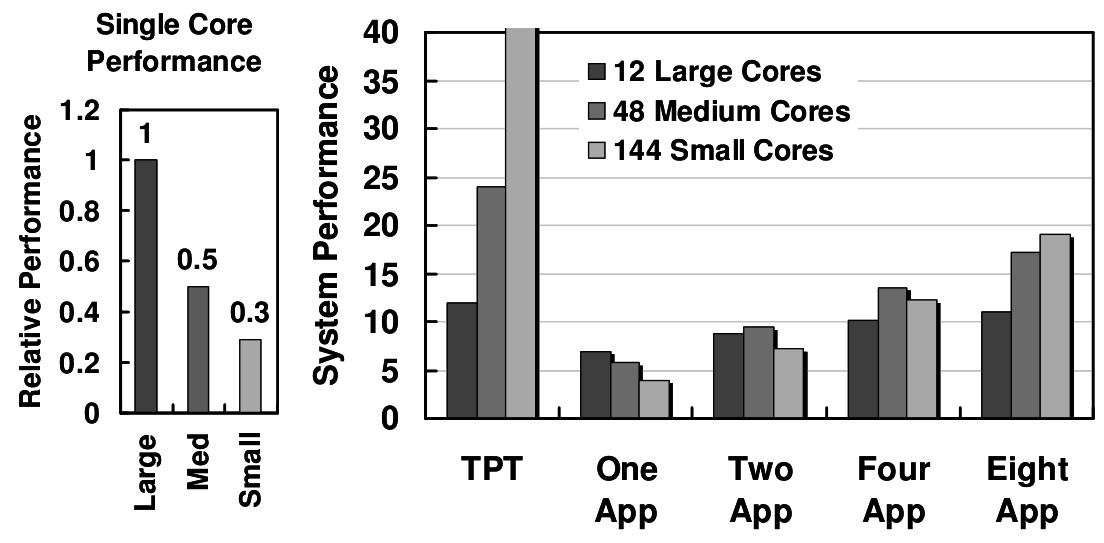
\includegraphics[width=0.5\textwidth]{images/pollack.png}
    \caption{Performance of Large, Medium and Small Cores}
    \label{fig:core_size_performance}
\end{figure}

However, application performance suffers from its serial factor, which is
formally described by Amdahl's law:

$$
\text{Parallel speedup} =
\frac{1}{\text{Serial \%} + (1 - \text{Serial \%}) / N}
$$

If serial percentage is large, then parallel speedup saturates with small number
of cores. Figure~\ref{fig:amdahl} illustrates the impact of serial
percentage of code on parallel speedup.

\begin{figure}[h]
    \centering
    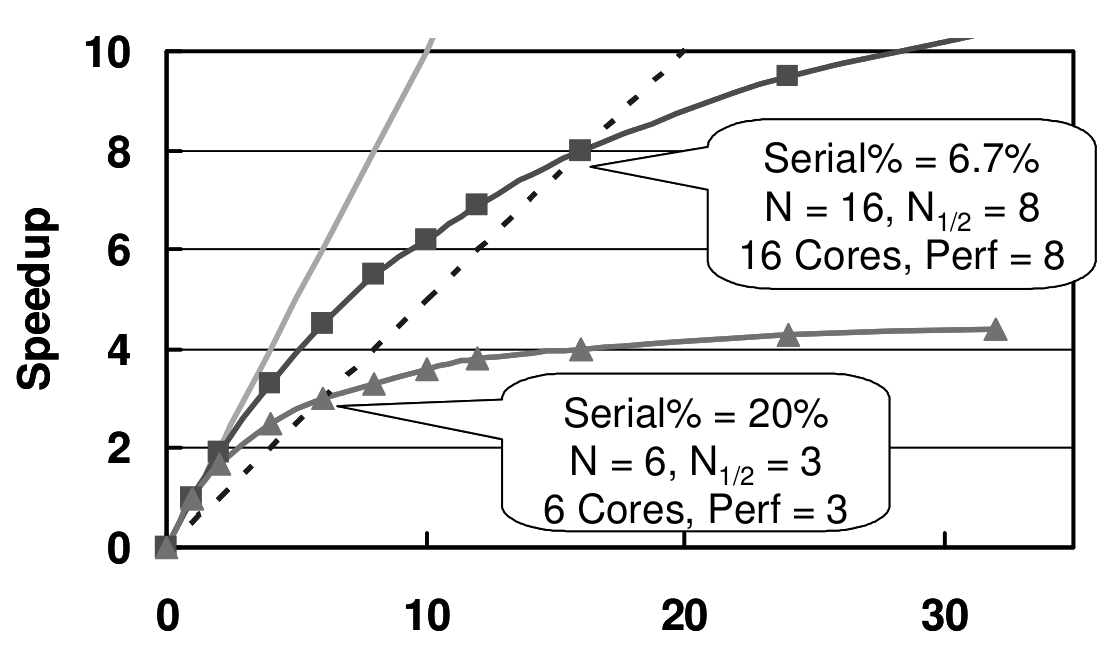
\includegraphics[width=0.5\textwidth]{images/amdahl.png}
    \caption{Amdahl's Law limits parallel speedup}
    \label{fig:amdahl}
\end{figure}

The conclusions are that it is very important to reduce serial part of the
program. In practice, it is complicated to get it right. We will come back to
this further in the report.

To sum up, this is where the future of microprocessors is heading to: having
more less powerful cores to do the work\cite{future-microprocessors}, and
programming languages and tools are developed to make parallel programming
easier, i.e. to reduce the serial component.

\subsection{Inter-core communication}

In current systems data exchange between cores is handled via shared memory,
while maintaining the coherency of the CPUs caches. Conversely, Tilera employed
a faster approach alongside: a high-bandwidth low-latency switched network
between the cores, which can be used by applications for very fast and low
latency data exchange directly between the CPUs\cite{tile64}.

From functional perspective, this kind of many-core system in many aspects
resembles a many-node cluster. Machines (tiles) communicate with each other by
sending messages; machines (tiles) can fail; they have to synchronize their
actions (think about locks and mutexes, which are much more complicated without
having shared memory). Since message-passing based many-core chips are coming to
the stage, it is important to investigate consensus algorithms in many-core
systems.

\section{Consensus and Paxos family overview}
\label{sec:paxos-family}

Paxos family algorithms are designed for reliably reaching a consensus in a
distributed system. The most primitive application is reliably learning a value
by a majority of acceptors. It works as follows: a set of proposers propose a
value, and the algorithm guarantees that only one value will be chosen by a
majority of acceptors. In worse case no value will be chosen.

The most popular application is distributed state machine implementation
\footnote{\url{http://en.wikipedia.org/wiki/Paxos\_(computer\_science)}}. A
majority of cluster nodes can use this algorithm to agree on an order in which
to execute a series of commands. A classical example for this is database
transaction synchronization across many database nodes, which have local copies
of data. State machine replication is built on the primitive of choosing a
single value.

Paxos algorithms are used primarily for synchronizing distributed systems. A few
notable examples: Google uses Paxos in their distributed locking service
Chubby\cite{chubby} (which is an important building block of BigTable). Another
example is OpenReplica\cite{openreplica}, where Paxos is used to implement a
replicated state machine.

\cite{paxos-simple} explains the classical way to implement a replicated state
machine:

\begin{quote}
To guarantee that all servers execute the same sequence of state machine
commands, we implement a sequence of separate instances of the Paxos consensus
algorithm, the value chosen by the $i^{th}$ instance being the $i^{th}$ state
machine command in the sequence.
\end{quote}

While this is simple and reliable, sometimes is inefficient. Two commands issued
in parallel can \emph{interfere} or \emph{commute}. \emph{Commute} means the
order of execution does not matter; likewise, \emph{interfering} commands must
be executed in the same order. For example, the order of two \emph{deposit}
operations on the same account does not matter, so these two commands
\emph{commute}. Likewise, two commands always commute if they are executed on
different accounts. However, \emph{deposit} and \emph{withdrawal} of the same
account must be executed in the same order as they can produce different
outcomes (negative balance) if executed in different orders.

In many systems, concurrently issued commands almost always commute. An
implementation that saves a message delay in almost all cases can be
significantly more efficient than one using the conventional state-machine
approach\cite{generalized-consensus}. For that reasons generalized consensus is
important.

Generalized Consensus and Paxos generalizes state-machine replication by
reaching an agreement on a partially ordered set of commands.

\fggc\ improves Generalized Consensus and Paxos in case of collision from six
message delays to one.

\subsection{Overview of Fast Genuine Generalized Consensus (FGGC)}

From abstract\cite{fggc}:

\begin{quote}
Consensus is a central primitive for building replicated systems, but its
latency constitutes a bottleneck. A well-known solution to consensus is Fast
Paxos. In a recent paper, Lamport enhances Fast Paxos by leveraging the
commutativity of concurrent commands. The new primitive, called Generalized
Paxos, reduces the collision rate, and thus the latency of Fast Paxos. However
if a collision occurs, the latency of Generalized Paxos equals six communication
steps, which is higher than Fast Paxos. This paper presents FGGC, a novel
consensus algorithm that reduces recovery delay when a collision occurs to
one.
\end{quote}

We want to implement FGGC, because it is the most flexible version to implement
a realistic state machine in Paxos, and is the fastest (least message delays)
generalized version that we are aware of as of time of the work.

\subsection{Language Choice}
\label{sec:erlang-why}

The language decision was based on these factors:
\begin{enumerate}
    \item It can run on Tilera64.
    \item How well is it suitable for parallel algorithm implementation.
    \item Performance.
\end{enumerate}

Initially Haskell was chosen for the algorithm implementation, for the following
reasons. It is very convenient to program state machines in a functional
language; it compiles to machine code, which makes it a good candidate for
performance. Furthermore, llvm compiler looked like a promising sign for
portability.

However, after some research it turned out that cross-compilation is impossible,
and the whole GHC must be ported to Tilera platform. Porting GHC to Tilera was
out of the scope of the project, so other languages were considered.

Another language candidate was Erlang. Erlang is a general-purpose, concurrent,
and functional programming language developed by Engineers from Ericsson in
1980s. Erlang is a language based on the  {\em actor model}, characterized by
the following features:

{\em Concurrency:} Erlang has extremely lightweight processes whose memory
requirements can vary dynamically. Processes have no shared
memory\footnote{They do in some circumstances for efficiency reasons, but this
is completely transparent to the programmer} and communicate by asynchronous
message passing.

{\em Distribution:} Erlang is designed to be run in a distributed
environment: it is as easy to create a process and communicate to
it on a host node like on a remote node.

The most appealing feature of Erlang is its approach to concurrency. Erlang {\em
actors} and message passing are higher-level synchronization primitives than
mutexes and condition variables. User can spawn millions of processes in Erlang
VM and Erlang will do a very good job in parallelizing their work with extremely
low context-switching and message passing overhead.

Erlang is written in C and requires standard UNIX tools to (cross-)compile and
run it. Supported platforms includes any Unix system, vxworks, Linux and
Windows
\footnote{\url{http://www.erlang.org/doc/installation\_guide/INSTALL.html}}.
Older version of Erlang (R13B) has been cross-compiled and ran on Tilera
Multi-core Development Environment (MDE) version 2. Some patches to the build
system were necessary to compile newer version of Erlang (R15B02) on the
version 3 of Tilera MDE. They have been submitted upstream.

\subsection{About Erlang Run Time System (ERTS)}

Under the hood Erlang virtual machine is a bytecode interpreter\footnote{for x86
systems there is an optional native code compiler \emph{hipe}\cite{hipe}, which
aims to improve computational performance}. Erlang itself is an OS process,
which main building parts are {\em schedulers} and {\em processes}. Erlang
processes are light-weight (grow and shrink dynamically) with small memory
footprint, fast to create and terminate and the scheduling overhead is low.
These are scheduled by Erlang run-time system. {\em Scheduler} is an OS thread
which schedules the Erlang processes. By default Erlang creates as many
schedulers as there are cores available. On Linux Erlang uses information about
CPU topology to exploit data locality.

An Erlang {\em node} is an Erlang VM instance which can talk to other nodes.
Several nodes can be on different machines. Nodes can communicate over TCP, SSL
and unix pipes (default and most popular is TCP). Processes within a node can
transparently send messages to other processes (semantics are the same as if
they were sent from the same node), monitor other nodes or processes.

\section{About TILEPro64}
\label{sec:tilera}

\begin{figure}
    \centering
    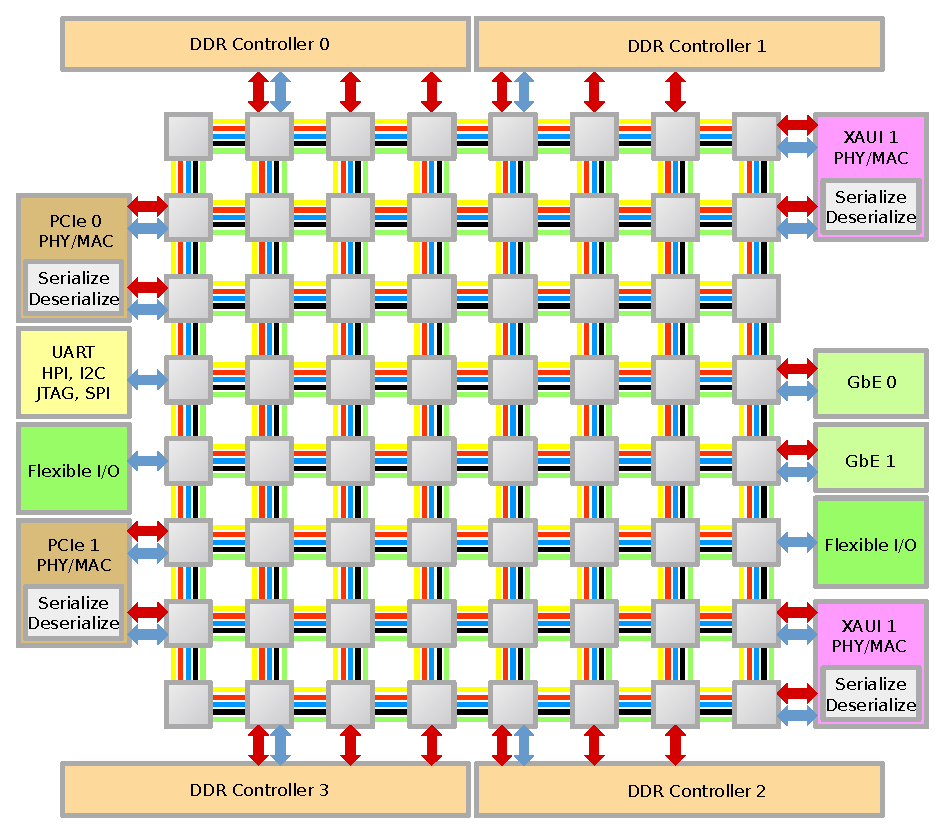
\includegraphics[width=0.5\textwidth]{images/tile64.pdf}
    \caption{TILEPro64 processor network block diagram}
    \label{fig:tile64}
\end{figure}

Figure~\ref{fig:tile64} is the block diagram of TILEPro64 processor. It consists
of a mesh network of 64 {\em tiles}, where each {\em tile} houses a general
purpose processor, cache, and a non-blocking router, which the tile uses to
communicate with the other tiles on the processor.

There is high-speed, low-latency packet-switched network between the cores for a
few purposes. Most interesting are two: shared L3 cache and User Dynamic
Network, UDN.

\subsection{Shared L3 cache}

\begin{figure}
    \centering
    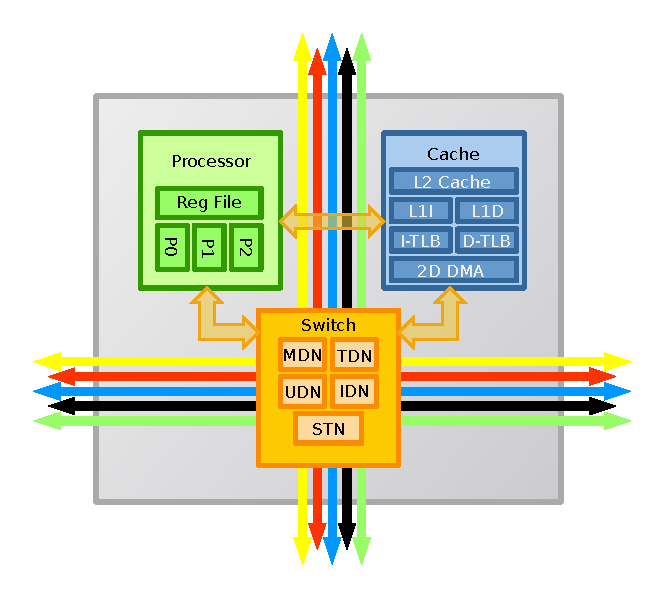
\includegraphics[width=0.5\textwidth]{images/tile64_cpu.pdf}
    \caption{TILEPro64 single processor diagram}
    \label{fig:tile64_cpu}
\end{figure}

Like seen in figure~\ref{fig:tile64_cpu}, every tile has three caches: L1D, L1I
and L2. L2 cache size is 64KiB. L3 is a "virtual cache" shared between tiles,
which size is 64KiB * 64 = 4MiB, thus creating 4 MiB of quickly accessible
on-chip cache.

\subsection{User Dynamic Network (UDN)}

Tilera has very interesting feature: User Dynamic Network, UDN. It is very low
latency (sending 130B message takes in the order of ticks) and high bandwidth
(order of tens of gigabits per second) switched inter-core network.

It can be very interestingly exploited in message-passing systems for
low-latency communication. Example of successful usage of this network is
presented in section~\ref{sec:future-work}.

\subsection{One or more Linux instances simultaneously}

TILEPro64 can run multiple Linux SMP instances on different tile configurations
(1-64 cores per Linux instance). In this project we run single Linux SMP
instance with 62 dedicated cores.

\section{Erlang evaluation on Tilera64}
\label{sec:erlang-eval}

\subsection{Related work}

A good example of a very robust synchronization between cores implementation
using message passing is memcached port to Tilera done by Facebook. UDN was used
for action orchestration and state synchornization\cite{facebook-tilera}. That
yielded impressive performance compared to standard architecture servers.

Interest in suitability of software development with Erlang on multi-core
processors is increasing. For instance, Convey et~al.\cite{erlang-acoustic}
investigate the relative merits of C++ and Erlang in the implementation of a
parallel acoustic ray tracing algorithm. Marr et~al.\cite{vm-manycore} analyze
virtual machine support for many-core architectures including Erlang.

Jianrong \cite{erlang-manycore-scalability} analyzes performance characteristics
of Erlang virtual machine on Tilera64. The paper focused on benchmarking
\emph{embarrassingly parallel} programs (ones that can run without a need for
synchronization with each other). It achieved speedups of 30-40 by using 64
cores.

Project UPMARC\footnote{\url{http://www.it.uu.se/research/upmarc}} creates tools
that improve testing of many-core systems development. Number of them are
implemented in/for
Erlang/OTP
\footnote{\url{http://www.it.uu.se/research/upmarc/publications/researchers}}.

\begin{quote}
UPMARC's goal is to develop the insights that enable new tools and approaches to
make parallel programming easier, and to demonstrate their effectiveness through
prototype implementations on real problems.
\end{quote}

\begin{quote}
RELEASE\footnote{\url{http://www.release-project.eu/}} is an EU FP7 STREP
(287510) project that aims to scale the radical concurrency-oriented programming
paradigm to build reliable general-purpose software, such as server-based
systems, on massively parallel machines. The trend-setting language we will use
is Erlang/OTP which has concurrency and robustness designed in. Currently
Erlang/OTP has inherently scalable computation and reliability models, but in
practice scalability is constrained by aspects of the language and virtual
machine. Moreover existing profiling and debugging tools don't scale.
\end{quote}

\subsection{Erlang parallelism performance on TILEPro64}

Performance of Erlang on TILE64 with a program that does no synchronization
between the workers was tested. It works as follows: $Master$ process generates
$N$ lists with 100000 random numbers (where $N$ is number of workers) and spawns
a new $Worker$ process passing the generated list. Once all workers are spawned,
$Master$ sends a message to all the workers to {\tt begin work}. When $Master$
process receives a number from every worker, the program terminates.

$Worker$ process: it receives {\tt begin work} message, sorts the list and
sends median to the $Master$. Then terminates. Pseudocode:

\begin{algorithm}
    \begin{algorithmic}
        \Function{Master}{}
            \State $PidList \gets []$
            \State $N \gets 128$
            \For{every $N$}
                \State $L \gets$ list of 100000 random numbers
            \EndFor
            \State $Pid \gets spawn(Worker, L)$
            \Comment{spawn $Worker$ process and pass $L$ to it}
            \State Append $Pid$ to $PidList$
            \State $StartTimestamp \gets now()$
            \Comment{Start measuring execution time}
            \For{$Worker$ in $PidList$}
                \State $Worker$ ! {\tt 'begin work'}
                \Comment{send {\tt 'begin work'} to $Worker$}
            \EndFor
            \For{$Worker$ in $PidList$}
                \State receive $\_Number$
                \Comment{receive $\_Number$ (which is a median of some list) and
                discard it}
            \EndFor
            \State print $Delta \gets now() - StartTimestamp$
        \EndFunction

        \Function{Worker}{$L$}
            \Comment{note that worker receives $L$ on startup (big list)}
            \State receive {\tt 'begin work'}
            \Comment{wait until {\tt 'begin work'} is received from master}
            \State $L2 \gets sort(L)$
            \State $Master$ ! $median(L2)$
            \Comment{send median of $L2$ to $Master$}
        \EndFunction
        \Comment{at this point $Worker$ process terminates}
    \end{algorithmic}
    \caption{pseudo-code of embarrassingly parallel program}
    \label{alg:embarrassing}
\end{algorithm}

\subsubsection{Serial component in embarrassingly parallel program}

Note that this program actually has a serial component it's the sending messages
{\tt begin work} and gathering the median to the single process. To check the
real cost of it, a similar program was created to check just process spawning
and message sending overhead. It works the same way like
program~\ref{alg:embarrassing}, but instead of passing a list and an item, {\tt
ok} is passed to process and back. Master process creates 100000 workers, sends
each of them its {\em pid} and waits for 100000 {\tt ok}'s. Worker process
replies to the {\em pid} it received with an {\tt ok}.

On Intel Core Duo CPU @ 1.66GHz the whole process takes 0.85-0.9 seconds, or up
to $9\mu s$ per process. So the serial overhead of program~\ref{alg:embarrassing}
is not more than $9*256 = 2304 \mu s$, or no more than two and a half
milliseconds. With 1 core program\ref{alg:embarrassing} runs for around 5
minutes, so 2.5 milliseconds of serial component is overwhelmed by actual work
of the workers and can be neglected.

\subsection{Embarrassingly parallel program scalability and VM tuning}

We would expect this program to scale linearly while increasing number of cores.
Initial results of the benchmarks are shown in figure~\ref{fig:bad_speedup}.
The maximum speedup is around 12 with a spike to 14, and the results are very
unstable when increasing the number of cores. To summarize, initial benchmarks
show that Erlang VM without tuning on a many-core machine performs poorly.

\begin{figure}
    \centering
    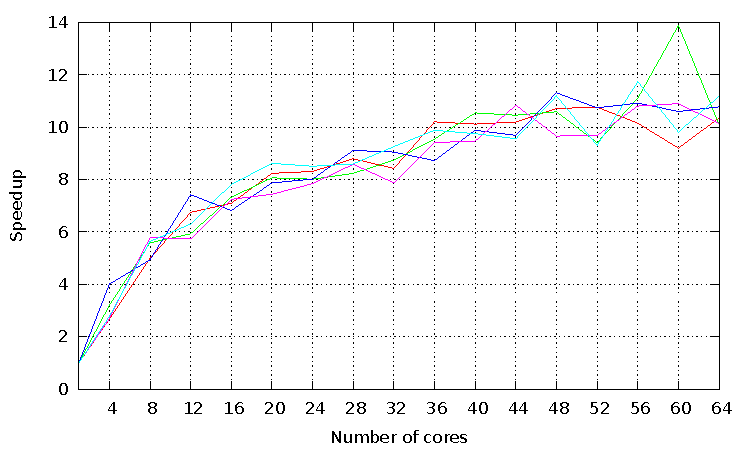
\includegraphics[width=0.9\textwidth]{images/bad_speedup.pdf}
    \caption{Initial speedup of algorithm~\ref{alg:embarrassing} (5 measurements)}
    \label{fig:bad_speedup}
\end{figure}

Kenneth Lundin gave a talk in Erlang Factory\cite{lundin-smp} about Erlang
many-core performance and suggested to pin Erlang schedulers (OS threads) to
hardware cores. This can be achieved by passing {\tt +sbt db} flag on during
startup of the Erlang virtual machine. This adjustment gave significant
improvement: performance stabilized and jumped to around 37 for 56 cores, as
shown in figure~\ref{fig:parallel_speedup}.

\begin{figure}
    \centering
    \includegraphics[width=0.9\textwidth]{images/speedup.pdf}
    \caption{Speedup of algorithm~\ref{alg:embarrassing}}
    \label{fig:parallel_speedup}
\end{figure}

\begin{figure}
    \centering
    \includegraphics[width=0.9\textwidth]{images/slowdown.pdf}
    \caption{Slowdown of algorithm~\ref{alg:embarrassing} (derived
    from figure~\ref{fig:parallel_speedup})}
    \label{fig:parallel_slowdown}
\end{figure}

Figure~\ref{fig:parallel_slowdown} is derived from~\ref{fig:parallel_speedup}
and shows precisely the loss of speedup while increasing the number of cores.

This experimental data shows that Erlang scales pretty well with increasing
number of cores. More details about it can be found in work by
Jianrong\cite{erlang-manycore-scalability}.

Currently in Erlang message sending between processes is implemented using
shared memory, locks and mutexes. However, it would be a very interesting
project to replace inter-erlang-process communication with UDN thus eliminating
the shared memory. Most importantly, application developer would not notice the
usability change; however, this would potentially eliminate a lot of bottle-neck
during message passing which incurs by going out of chip.

\section{FGGC in Erlang}
\label{sec:paxos-api}

Implementation of FGGC should be done in this order:

\begin{enumerate}
    \item Classic paxos.
    \item State machine using classic paxos.
    \item Generalized Paxos.
    \item GPaxos.
    \item \fggc.
\end{enumerate}

Every step is a pre-requisite for the next one. There are three Classic Paxos
implementations in Erlang \footnote{\url{https://github.com/gburd/gen\_paxos}}
\footnote{\url{http://libpaxos.sourceforge.net/paxos\_projects.php\#erlangpaxos}}
\footnote{\url{http://code.google.com/p/scalaris/}}, but they are written in a
way that it will be very difficult to extend the algorithm. Therefore classic
paxos has been reimplemented.

\subsection{Clasic Paxos in Erlang}

Here is the API of classic paxos:

\begin{verbatim}
-type fsmref() :: reference().
-type value() :: term().
-type learner_callback() :: fun((value()) -> ok).

%% @doc Specify learner function per election.
%% The passed function will be executed when a value is learned.
-spec init_learner(fsmref(), learner_callback()) -> ok.

%% @doc Executed by application in order to propose a value
-spec propose(fsmref(), value()) -> ok.
\end{verbatim}

To propose a value, application calls {\tt propose()}. When the value (same or
other one) is learned, user's callback {\tt learn()} is called.

{\tt fsmref()} is an \emph{election} and \emph{electorate} identifier. It is
acquired during the start-up of proposers, acceptors and learners; in this work
we are not concerned about the start-up of the cluster and how this value is
generated.

\subsection{State machine replication API using Classic Paxos}

Once Classic Paxos is done, Paxos state machine can be implemented. The API is
very similar, but {\tt id()} is associated with every election (election id):

\begin{verbatim}
-type id() :: pos_integer().
-type learner_callback() :: fun((fsmref(), id(), value()) -> ok).

%% @doc Specify learner function per election.
%% The passed function will be executed when a value is learned.
-spec init_learner(fsmref(), learner_callback()) -> ok.

%% @doc Executed by application in order to propose a value
-spec propose(fsmref(), id(), value()) -> ok.
\end{verbatim}

With these two functions user is able to implement a replicated state machine.
However, like observed before, in most systems different commands issued in
parallel are converging, i.e. can be executed in any order.

To overcome this inefficiency, we present the generalized API.

\subsection{State machine replication API using Generalized Paxos}

\begin{verbatim}
-type id() :: pos_integer().
-type command() :: term().

-type learner_callback() :: fun((fsmref(), id(), value()) -> ok).
-type commands_commute() :: fun((command(), command()) -> boolean()).

%% @doc Specify learner function and command comparison fun per election.
-spec init_learner(fsmref(), learner_callback(), compare_commands()) -> ok.

%% @doc Executed by application in order to propose a value
-spec propose(fsmref(), [id()], [value()]) -> ok.
\end{verbatim}

Note to Wim: {\tt propose/3} API most likely does not make sense.

\section{Conclusion}
\label{sec:conclusion}

This paper presents the suitability of Erlang for algorithm implementation on
many-core machines and suggests an API for state machine replication using
\fggc.

\subsection{Future work}
\label{sec:future-work}

Implementation of FGGC and performance evaluation on heterogeneous cluster is
left for future work. Also using UDN for message passing in Erlang virtual
machine would also be a very interesting project.

\subsection{Acknowledgement}

The author thanks Wim Vanderbauwhede for his comments and continuous support in
all phases of this personal project.

\clearpage
\begin{thebibliography}{99}

    \bibitem{fggc} Sutra,~P. \emph{Fast Genuine Generalized Consensus}. Reliable
        Distributed Systems (SRDS), 2011 30th IEEE Symposium.

    \bibitem{hipe} Sagonas,~K., Wilhelmsson,~J. \emph{Efficient memory
        management for concurrent programs that use message passing}. Science of
        Computer Programming, 62(2): p.~98-121, October 2006.

    \bibitem{1kcorechips} Borkar,~S. \emph{Thousand Core Chips—A Technology
        Perspective}. DAC '07 Proceedings of the 44th annual Design Automation
        Conference. p.~746-749.

    \bibitem{pollack} Pollack,~F. \emph{Pollack's Rule of Thumb for
        Microprocessor Performance and Area.}

    \bibitem{future-microprocessors} Borkar~S., Chien,~ A.~A. \emph{The Future
        of Microprocessors}. Communications of the ACM, Vol. 54 No. 5, p.~67-77.

    \bibitem{tile64} Bell,~S., Edwards,~B., Amann,~J., Conlin,~R.,
        Joyce,~K., Leung,~V., MacKay,~J., Reif,~M., Bao,~L., Brown,~J.,
        Mattina,~M., Miao,~Chyi-Chang, Ramey,~C., Wentzlaff,~D.,
        Anderson,~W., Berger,~E., Fairbanks,~N., Khan,~D., Montenegro,~F.,
        Stickney,~J., Zook,~J. \emph{TILE64 -- Processor: A 64-Core SoC with
        Mesh Interconnect}. Solid-State Circuits Conference, 2008. ISSCC 2008.
        Digest of Technical Papers. IEEE International. p.~88-598.

    \bibitem{classic-paxos} Lamport,~L. \emph{The part-time parliament}. ACM
        Transactions on Computer Systems (TOCS). Volume 16 Issue 2, May~1998.
        p.~133-169.

    \bibitem{paxos-simple} Lamport.,~L. \emph{Paxos made simple}. ACM SIGACT
        News (Distributed Computing Column) 32, 4 (Whole Number 121, December
        2001) p.~51-58.

    \bibitem{generalized-consensus} Lamport.~L. \emph{Generalized Consensus and
        Paxos}. Microsoft Research Technical Report MSR-TR-2005-33.

    \bibitem{chubby} Burrows,~M. \emph{The Chubby lock service for
        loosely-coupled distributed systems}. OSDI '06 Proceedings of the 7th
        symposium on Operating systems design and implementation. p. 335-350.

    \bibitem{openreplica} Altinbuken,~D., Emin~Gun.,~S. \emph{Commodifying
        Replicated State Machines with OpenReplica}. Computing and
        Information Science Technical Reports, Cornell University.

    \bibitem{erlang-acoustic} Convey,~C., Fredricks,~A., Gagner,~C.,
        Maxwell,~D., Hamel,~L. \emph{Experience report: erlang in acoustic ray
        tracing}. In ICFP ’08: Proceeding of the 13th ACM SIGPLAN international
        conference on Functional programming, pages 115–118, New York, NY, USA,
        2008. ACM.

    \bibitem{vm-manycore} Marr,~S. D’Hondt,~T. \emph{Many-core virtual machines:
        decoupling abstract from concrete concurrency}. In SPLASH ’10:
        Proceedings of the ACM interna- tional conference companion on Object
        oriented programming systems languages and applications companion.
        p.~239–240, New York, NY, USA, 2010. ACM.

    \bibitem{erlang-manycore-scalability} Jianrong, Z. \emph{Characterizing the
        Scalability of Erlang VM on Many-core Processors}. Student thesis, KTH,
        School of Information and Communication Technology (ICT).

    \bibitem{facebook-tilera} Berezeckia,~M., Frachtenberga,~E. Palecznya,~M.
        Steeleb,~K. \emph{Power and performance evaluation of Memcached on the
        TILEPro64 architecture}. Sustainable Computing: Informatics and Systems.
        Volume 2, Issue 2, June 2012, p. 81–90.

    \bibitem{amdahls-law} Hill,~Mark~D. \emph{Amdahl's Law in the Multicore
        Era}. Dept. of Comput. Sci., Univ. of Wisconsin-Madison, Madison, WI
        Marty, Michael R.  Vol.~41, Issue~7. p.~33-38.

    \bibitem{lundin-smp} Lundin,~K. \emph{About Erlang/OTP and Multi-core
        performance in particular}. Talk at Erlang Factory London June 26 2009.


\end{thebibliography}

\educationalconsent

\end{document}
